\subsection{MLL-AF4 and cooperative TFs co-opt and drive normal fetal circuits.}

MLL-AF4 and RUNX1 function cooperatively at many loci, and co-regulated genes are enriched for B cell differentiation processes (Fig. \ref{fig:ch4_interplay}B). As \textit{MLL} translocations are thought to occur in fetal life \citep{greaves_causal_2018, greaves_utero_2005, ford_utero_1993, jackson_origin_2021}, and the MLL-AF4 GRN has FBM active modules (See Fig. \ref{fig:ch4_patient}), it is possible MLL-AF4 uses fetal TFs to co-opt normal fetal pathways. In collaboration with the Roy lab, we generated single cell RNA+ATAC multiome (sc-multiome) data profiling healthy CD34+ (stem) and CD34- FBM and fetal liver (FL) from healthy donors. In addition, we profiled iALL and chALL blasts from patients, alongside xenograft models of MLL-AF4 transformed cord blood generated by Siobhan Rice using CRISPR induced translocation \citep{rice_human_2021} (Table \ref{tbl:ch4_multiome-samples}). Samples were multiplexed in male-female pairs (see deconvolution methods). High quality, and robustly deconvoluted cells were retained, and the iALL-X and chALL-X samples were discarded for poor cell capture (Table \ref{tbl:ch4_multiome-samples}, Appendix. \ref{fig:app_multiome-qc}A-C).

\begin{table}[htbp]
\resizebox{\textwidth}{!}{
\begin{tabular}{@{}llllllll@{}}
\toprule
ID & Patient & Population & Gender & Well & Cells pre-QC & Cells post-QC & Notes \\ \midrule
FBM1.1 & ICH13451 & CD34- FBM & Male & 1 & 3836 & 3146 &  \\
FBM2.1 & ICH15633 & CD34- FBM & Female & 1 & 3810 & 2966 &  \\
FBM1.2 & ICH13451 & CD34+ FBM & Male & 2 & 3748 & 3359 &  \\
FBM2.2 & ICH15633 & CD34+ FBM & Female & 2 & 3123 & 2567 &  \\
FL1.1 & ICH13451 & CD34- FL & Male & 3 & 3276 & 2736 &  \\
FL2.1 & ICH15633 & CD34- FL & Female & 3 & 3165 & 2611 &  \\
FL1.2 & ICH13451 & CD34+ FL & Male & 4 & 3129 & 2735 &  \\
FL2.2 & ICH15633 & CD34+ FL & Female & 4 & 4998 & 4180 &  \\
iALL2 & 28349 & iALL blasts & Male & 5 & 3901 & 3518 &  \\
iALL1 & 874415 & iALL blasts & Female & 5 & 3653 & 2868 &  \\
iALL3 & 863388 & iALL blasts & Male & 6 & 5435 & 4526 &  \\
chALL & 26754 & chALL blasts & Male & 6 & 5755 & 5160 &  \\
chALL-X & 23003 & chALL blasts & Male & 7 & 474 & 30 & Fail \\
iALL-X & 11911 & iALL blasts & Female & 7 & 595 & 350 & Fail \\
Xeno2-1 & 14428 & xenoALL blasts & Male & 8 & 2856 & 2512 &  \\
Xeno3-3 & 15254 & xenoALL blasts & Female & 8 & 3018 & 2724 &  \\
Xeno2-2 & 14428 & xenoALL blasts & Male & 9 & 4994 & 4530 &  \\
Xeno3-2 & 15254 & xenoALL blasts & Female & 9 & 6196 & 5752 &  \\
Failed deconvolution &  &  &  &  & 8841 &  &  \\ \bottomrule
\end{tabular}
}
\caption{Patients and donor samples used for single cell RNA+ATAC multiome analysis}
\label{tbl:ch4_multiome-samples}
\end{table}

FBM/FL samples and MLL-AF4 ALL blasts were clustered, incorporating both RNA expression and chromatin accessibility profiles (See methods, \cite{hao_integrated_2021}). Cells were annotated by label transfer using reference datasets \citep{popescu_decoding_2019, jardine_blood_2021, roy_transitions_2021}, and manually curated based on known B progenitor markers (Fig. \ref{fig:ch4_multiome-clusters}A-B, Appendix \ref{fig:app_multiome-lineage-markers}). Slingshot trajectory analysis grouped cells into three lineages originating from HSCs (Defined by \textit{HLF} expression, \cite{lehnertz_hlf_2021}), including erythropoiesis (\textit{HBB}), myelopoiesis/neutrophils (\textit{MPO}, \cite{aratani_myeloperoxidase_2018}), and B lymphopoiesis (\textit{PAX5}, \cite{nutt_pax5_2001}) (Fig. \ref{fig:ch4_multiome-clusters}C-D). As an artifact the erythropoiesis lineage also picks up an eosinophil/basophil/mast cluster (Eo-Ba-Ma, \textit{GATA2}, \cite{ohmori_gata2_2015}). Pseudotime ordering of these lineages organises cells into sequential clusters, from HSPCs through to mature populations (Fig. \ref{fig:ch4_multiome-clusters}E, Appendix \ref{fig:app_multiome-other-pseudo}).

\begin{figure}[htbp]
    \centering
    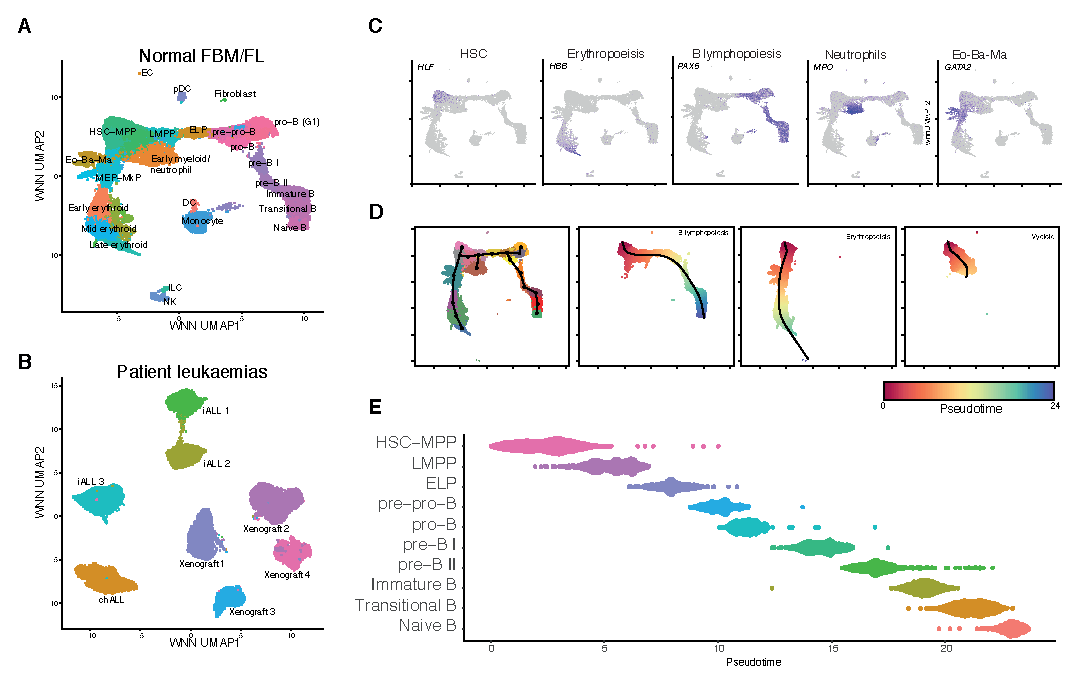
\includegraphics[width=\textwidth,height=\textheight,keepaspectratio]{figures/chapter4/ch4_multiome-clusters.png}
    \caption[{Sc-multiome trajectory analysis of  FBM and FL cells recapitulates three fetal lineages.}]
    {\textbf{Sc-multiome trajectory analysis of  FBM and FL cells recapitulates three fetal lineages.} 
    \textbf{(A, B)} UMAP dimensionality reduction and clustering performed using RNA+ATAC WNN graphs for normal FBM and FL cells (A), and patient and xenograft ALL blasts (B). Cluster identities annotated.
    \textbf{(C)} Expression of key lineage defining markers.
    \textbf{(D)} Lineage assignment through slingshot trajectory analysis, using HSC-MPP cluster as the lineage start.
    \textbf{(E)} B lymphopoiesis assigned cells ordered by slingshot pseudotime, stratified by assigned cluster as in A. 
    \textit{Analysis of the sc-multiome was performed by me in collaboration with Alastair Smith (scATAC-seq pre-processing and peak calling pipeline).}
    }
    \label{fig:ch4_multiome-clusters}
\end{figure}

Differential analysis for expression changing over pseudotime identified B lineage associated genes (see TradeSeq methods), which were clustered into six B lymphopoiesis signatures (B1-6, Fig. \ref{fig:ch4_multiome-tradeseq}A-B). As determined by single cell signature enrichment (AUcell), these map to HSC-MPP (B1), LMPP/ELP (B2), pre-pro-B/pro-B (B3), pre-B I and II (B4), immature/transitional B (B5) and Na\"{i}ve B (B6) cells (Fig. \ref{fig:ch4_multiome-tradeseq}C). Interestingly only signatures pre-pro-B/pro-B (B3), and to a lesser extent LMPP/ELP (B2), were enriched in iALL and chALL blasts (Fig. \ref{fig:ch4_multiome-tradeseq}D). This suggests that ALL blasts match transcriptional profiles from LMPP through to pro-B.

\begin{figure}[htbp]
    \centering
    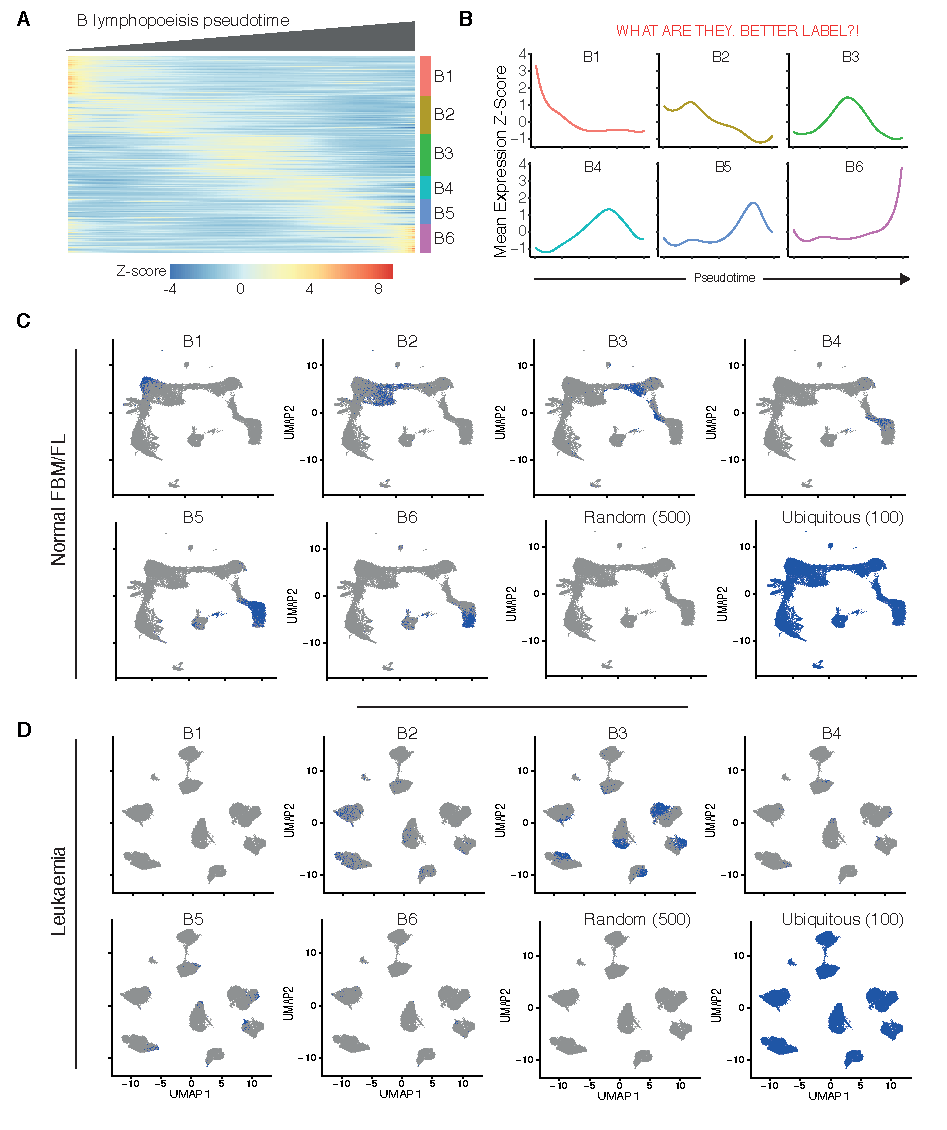
\includegraphics[width=\textwidth,height=\textheight,keepaspectratio]{figures/chapter4/ch4_multiome-tradeseq.png}
    \caption[{pre-pro-B/pro-B biased B-lymphopoiesis associated genes are enriched in MLL-AF4 ALL blasts.}]
    {\textbf{pre-pro-B/pro-B biased B-lymphopoiesis associated genes are enriched in MLL-AF4 ALL blasts.} 
    \textbf{(A)} Heatmap of z-score expression, smoothed over pseudotime into 100 bins, with genes as rows and cells as columns ordered by B lymphopoiesis pseudotime. \textit{k}-means clusters (B lymphopoiesis signatures) shown on the side.
    \textbf{(B)} Average z-score expression, smoothed over pseudotime into 100 bins, split by clusters as in A.
    \textbf{(C-D)} FL and FBM (C) or ALL blast (D) UMAPs, annotated with cells passing AUCell thresholds marking enrichment for signatures as in A-B. Same thresholds used for each signature between FBM/FL and ALL blasts, as well as random and ubiquitous gene sets.
    }
    \label{fig:ch4_multiome-tradeseq}
\end{figure}

To determine whether MLL-AF4 co-opts B lymphopoiesis circuits I integrated the MLL-AF4 GRN. MLL-AF4 regulated genes were more significantly associated with B lymphopoiesis over non-MLL-AF4 regulated genes, but this was not observed for erythropoiesis or myelopoiesis (neutrophils) (Fig. \ref{fig:ch4_multiome-grn}A). This aligns with the hypothesis that MLL-AF4 drives B progenitor circuits. 

Further, using the SEM \textit{MLL-AF4} KD logFC data to assign activating and repressing interactions (as in Fig. \ref{fig:ch4_motifs}), MLL-AF4 activated genes showed much greater B lymphopoiesis association than MLL-AF4 repressed genes (Fig. \ref{fig:ch4_multiome-grn}A). Strikingly, the GRN interfaces primarily with the B3 (pre-pro-B/pro-B) signature, and upon \textit{MLL-AF4} KD this signature, unlike others, is almost entirely downregulated (Fig. \ref{fig:ch4_multiome-grn}B-C). Distinguishing MLL-AF4 direct and indirect binding reveals most directly bound signatures are downregulated upon KD, whereas indirectly bound signatures are upregulated except for B3 (Fig. \ref{fig:ch4_multiome-grn}C). This can be interpreted as MLL-AF4 strongly activating a pre-pro-B/pro-B gene signature, both in the direct and indirect GRN, yet the indirect GRN may drive repression of stem and mature signatures. 

\begin{figure}[htbp]
    \centering
    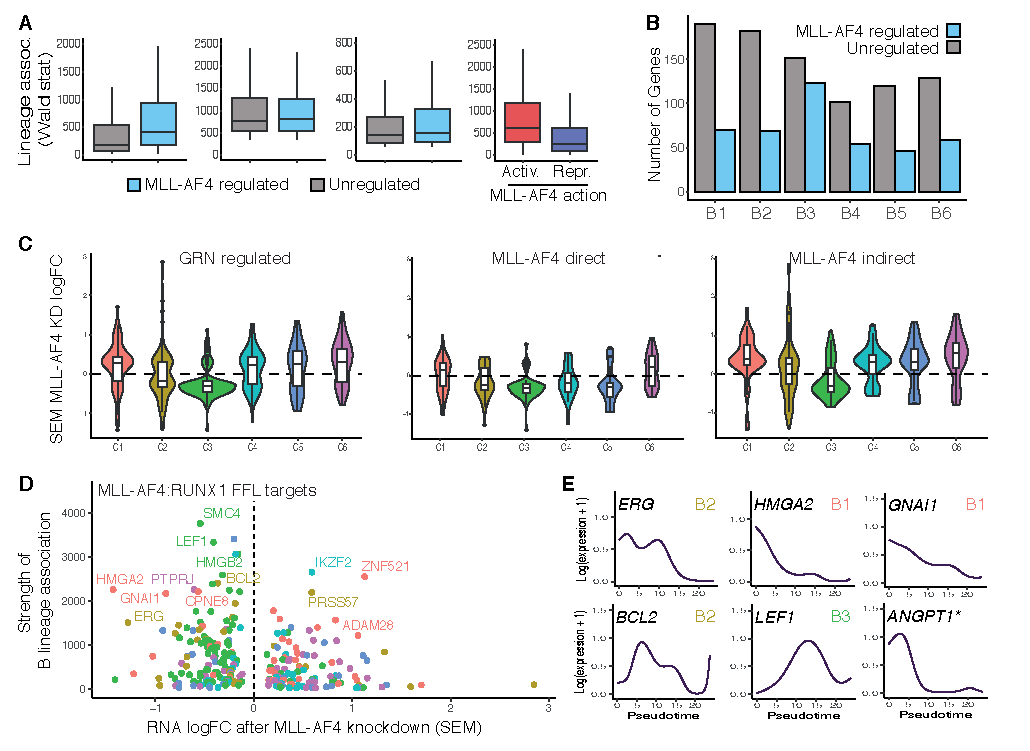
\includegraphics[width=\textwidth,height=\textheight,keepaspectratio]{figures/chapter4/ch4_multiome-grn.png}
    \caption[{The MLL-AF4 GRN drives activation of pre-pro-B/pro-B biased genes, and may repress mature B-cell circuits.}]
    {\textbf{The MLL-AF4 GRN drives activation of pre-pro-B/pro-B biased genes, and may repress mature B-cell circuits.} 
    \textbf{(A)} Distribution of TradeSeq Wald statistics of lineage association for genes expressed in different lineages, split by MLL-AF4 GRN regulation status.
    \textbf{(B)} Number of genes associated with each B lymphopoiesis signature, split by MLL-AF4 GRN regulation status.
    \textbf{(C)} Distribution of SEM RNA logFC following 96 hours' \textit{MLL-AF4} KD across B lymphopoiesis signatures at all GRN regulated genes, MLL-AF4 directly, and indirectly regulated genes. 
    \textbf{(D)} Relationship between SEM RNA logFC following 96 hours' \textit{MLL-AF4} KD and TradeSeq Wald statistic of lineage association for B lymphopoiesis. MLL-AF4:RUNX1 FFL motif targets shown. Genes annotated according to B lymphopoiesis signatures.
    \textbf{(E)} TradeSeq smoothed expression plots for select genes in D.
    }
    \label{fig:ch4_multiome-grn}
\end{figure}

A number of B lymphopoiesis associated genes are regulated by an MLL-AF4:RUNX1 driven FFL (Fig. \ref{fig:ch4_multiome-grn}D). Several FFL targets are associated with B lymphopoiesis, and are strongly regulated by MLL-AF4 (Fig. \ref{fig:ch4_multiome-grn}D-E). These include the key MLL-AF4 target \textit{BCL2}, which shows a B2 expression pattern (ELP/LMPP). \textit{LEF1} is a pre-pro-B/pro-B expressed gene that is a target of MLL-AF4 \citep{kerry_mll-af4_2017} and has a known role in driving pro-B proliferation as a part of WNT signalling \citep{reya_wnt_2000}. \textit{Lef1} was also highlighted in Maf:Lef1:EMT FFLs in mouse EHT (Fig. \ref{fig:ch3_maf1-lef1}). One interesting hypothesis is that MLL-AF4 drives the reactivation of stem and progenitor programs, as seen with the overexpression of \textit{PROM1} \citep{godfrey_h3k79me23_2021, mak_mixed_2012, obyrne_discovery_2019}. In line with this, we find \textit{HMGA2} and \textit{GNAI1} matching a HSC-MPP signature (B1), and \textit{ANGPT1} as detected by a specific HSC-MPP and pro-B differential test. This could reflect reactivation or forced maintenance of these loci. 

One factor of interest is \textit{ERG}, expressed in an ELP/LMPP biased signature (B2), that is expressed up until pro-B and downregulated in pre-B cells. Pseudo-bulked accessibility profiles of ALL blasts match pre-pro-B and pro-B cells, and is bound by spreading MLL-AF4 and RUNX1 in SEM cells. This suggests MLL-AF4 and cooperative TFs bind to the accessible landscape in pro-B cells and prevents inactivation of the locus (Fig. \ref{fig:ch4_multiome-erg}A). There are two \textit{ERG} transcripts commonly expressed in haematopoietic cells, \textit{ERG2} (NM\_004449) and \textit{ERG3} (NM\_182918) \citep{bohne_epigenetic_2009}. Interestingly, MLL-AF4 and RUNX1 are only bound at the \textit{ERG2} transcript promoter, and only \textit{ERG2} transcripts are expressed (Fig. \ref{fig:ch4_multiome-erg}B), suggesting the MLL-AF4 drives a shift in \textit{ERG} isoforms, though the consequence of this is not clear. \textit{ERG} deletion is required for V-to-DJ recombination and progression from a pro-B to pre-B state \citep{sondergaard_erg_2019}, yet \textit{ERG} overexpression in mouse haematopoiesis also results in an expansion of pro-B cells and a partial pro-B to pre-B block \citep{tsuzuki_promotion_2011}. As such, ERG may be required for V-to-DJ recombination but must be downregulated thereafter, hence forced expression could contribute to an ALL B differentiation block. In fact, ERG ChIP-seq shows binding at the Na\"{i}ve B signature (B6) genes at a higher proportion than other signatures (Fig. \ref{fig:ch4_multiome-erg}C), suggesting downstream ERG interaction with mature B programs. Altogether, these analyses highlight the capacity for MLL-AF4, and cooperating TFs, to drive normal fetal circuits, reactivate stem and progenitor TFs, and may repress mature B-cell programs, leading to a block in differentiation.

\begin{figure}[p]
    \centering
    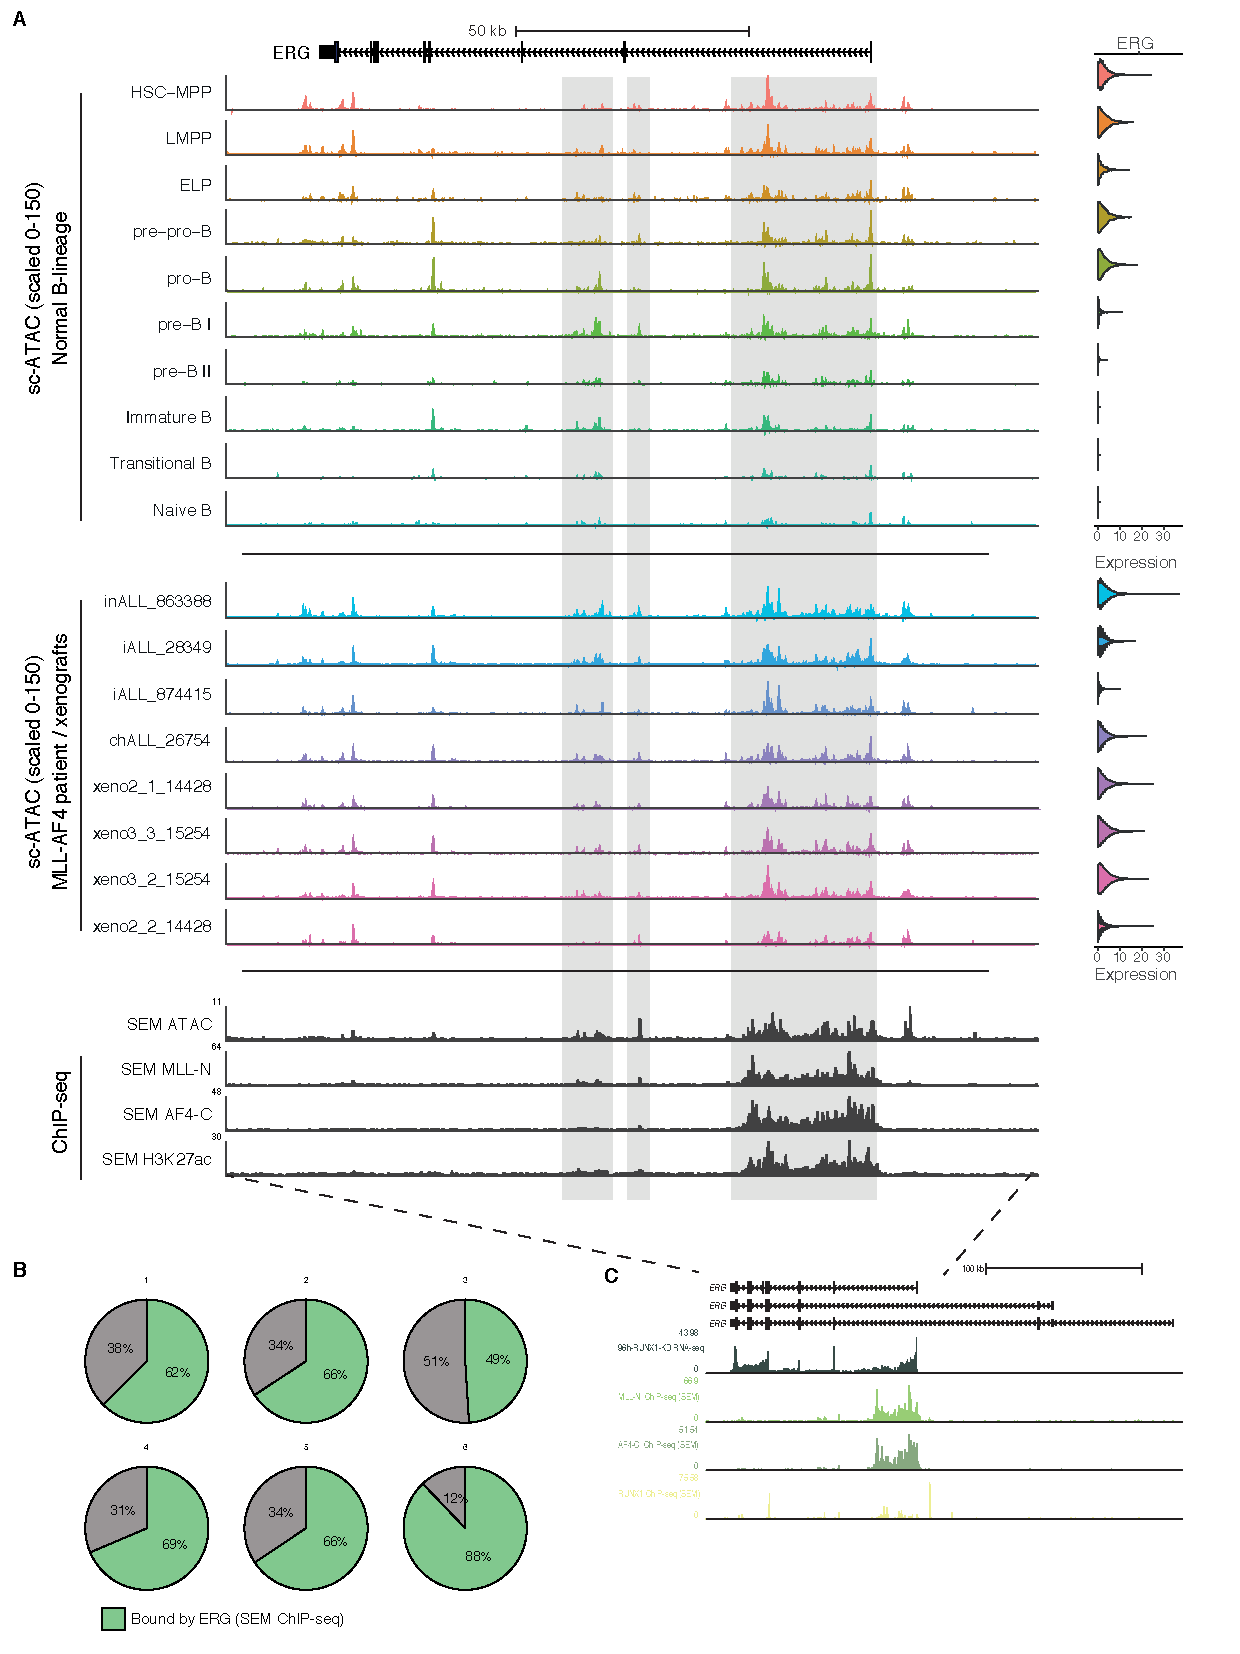
\includegraphics[width=0.9\textwidth,height=0.9\textheight,keepaspectratio]{figures/chapter4/ch4_multiome-erg.png}
    \caption[{MLL-AF4 and RUNX1 regulate a specific isoform of the fetal B-progenitor TF, \textit{ERG}.}]
    {\textbf{MLL-AF4 and RUNX1 regulate a specific isoform of the fetal B-progenitor TF, \textit{ERG}.} 
    \textbf{(A)} Panel of ATAC-seq and ChIP-seq tracks at the \textit{ERG} locus. scATAC-seq tracks are pseudobulked by cluster identity (FL/FBM) or sample identity (ALL blasts). Bulk ATAC-seq and ChIP-seq from SEM cells shown at the bottom. \textit{ERG} expression shown on the right.
    \textbf{(B)} Zoomed out tracks showing three \textit{ERG} isoforms, and SEM nascent RNA-seq and ChIP-seq.
    \textbf{(C)} Proportion of B lymphopoiesis signatures bound by ERG ChIP-seq.
    }
    \label{fig:ch4_multiome-erg}
\end{figure}

\subsection{TF cooperation in \textit{MLL}r promotes survival and leukaemogenesis}

The data thus far offers a breakdown of MLL-AF4 and TF cooperation in FFLs, and indirect MLL-AF4 regulation using TFs as intermediates in cascade motifs, that co-opt B progenitor circuits. MLL-AF4 and RUNX1 cooperative drive regulation of cell death and cell cycle processes (Fig. \ref{fig:ch4_interplay}B), so I investigated network motifs regulating these leukaemogenic features.